\section{Results}

\subsection{RQ1: Does Representation Alter Product Visibility?}

Figure~\ref{fig:crossmodel} answers the central question across datasets and retriever families. For the three general-purpose encoders, 9.41--13.26\% of highest-relevance WANDS pairs and 4.42--8.25\% of ESCI pairs cross the top-20 boundary under fact-equivalent attribute orders. Query-macro estimates are larger on WANDS (12.05--19.17\%) and remain 3.66--6.91\% on ESCI. Every macro confidence interval has a lower bound above the preregistered 1\% floor.



The detailed statistics in Supplementary Table S1 show that the WANDS crossings are not merely tie-breaking near rank 20. The median highest-relevance pair moves 81--207 positions across representations. ESCI has a different regime: median movements of two or three ranks for the general encoders still create consistent cutoff crossings because many judged products lie near the boundary. The e-commerce-specific retriever reduces WANDS micro VI@20 to 6.07\% but remains at 7.22\% on ESCI (Figure~\ref{fig:crossmodel}). Domain training therefore does not make serialization irrelevant.

\begin{figure}[t]
  \centering
  
\includegraphics[width=\columnwidth]{figures/figure2_cross_model_vi.pdf}
  \Description{Dot plots with confidence intervals compare query-macro visibility instability for four retrievers on WANDS and ESCI.}
  \caption{Equivalent attribute orders change visibility across general and e-commerce-specific retrievers. Error bars are 95\% query-bootstrap confidence intervals; the dashed line marks the 1\% preregistered floor.}
  \label{fig:crossmodel}
\end{figure}

Two checks narrow possible explanations. First, instability persists in the official ESCI candidate formulation. At top 10, micro VI is 7.60\%, 6.65\%, and 11.55\% for MiniLM, BGE, and GTE; at top 20 it is 3.00\%, 2.86\%, and 5.89\%. Because the median official pool contains 16 products, top-20 crossings are mechanically constrained. Condensed union-catalog NDCG equals official-pool NDCG after unjudged products are removed, so this is a visibility-formulation check rather than an independent effectiveness estimate. Second, changing chunk length, overlap, and pooling does not remove WANDS instability. MiniLM micro VI@20 remains 11.25--13.26\% across five profiles, BGE remains 9.41--17.77\%, and long-context GTE is also sensitive. A single short-context configuration cannot explain the pattern.

\paragraph{What the encoding controls rule out.}
Table~\ref{tab:encodingcontrols} expands the input-budget and pooling check. Every listed profile retains nonzero highest-relevance crossing, but the profiles do not preserve the same magnitude. In particular, chunking can increase BGE instability even while allowing more of a long record to contribute to its representation. More input coverage should therefore not be equated with order invariance. Window boundaries, within-window context, and aggregation all remain sensitive to how the record is presented.

\begin{table}[t]
\caption{WANDS catalog-wide encoding controls. Entries are pair-micro VI@20 percentages. Chunk sizes and overlap are in tokens; pooling specifies the within-chunk rule. These are configuration checks, not separately trained retrievers.}
\label{tab:encodingcontrols}\centering\small
\begin{tabular}{lrr}\toprule
Profile & MiniLM & BGE-base\\\midrule
Native & 13.26 & 9.41\\
Mean, chunk 126, overlap 32 & 12.10 & 14.45\\
Mean, chunk 254, overlap 0 & 11.72 & 17.63\\
Mean, chunk 254, overlap 64 & 11.25 & 17.77\\
CLS, chunk 254, overlap 0 & 11.63 & 17.15\\\bottomrule
\end{tabular}
\end{table}

These controls constrain the explanation without identifying a unique internal cause. The data reject the claim that the observed phenomenon disappears merely by choosing one of these alternative input configurations. They do not decompose the effect into truncation, positional encoding, attention, and pooling contributions. Changing several aspects of an encoding profile is not a clean intervention on any one of those mechanisms. Likewise, the long-context result broadens coverage but does not prove that truncation never matters for any individual record. The supported conclusion is configuration-robust evidence of representation sensitivity, rather than a complete mechanistic account of Transformer order effects.

\subsection{RQ2: Are Human-Relevant Products Materially Affected?}

The primary results already concern the highest relevance stratum: Exact products in WANDS and E products in ESCI. Figure~\ref{fig:example} demonstrates that an Exact item can move by 1,522 ranks while both its facts and all competitor representations remain fixed. At aggregate scale, WANDS shows more instability among Exact than Irrelevant pairs. The query-macro Exact-minus-Irrelevant difference is 17.01 percentage points for MiniLM, 10.90 for BGE, and 12.62 for GTE; the three 95\% intervals exclude zero and Holm-adjusted $p=.0003$. ESCI does not support the same gradient: E-minus-I differences range from $-0.41$ to $+1.63$ points, all intervals include zero, and adjusted $p\geq .4707$. The defensible cross-dataset conclusion is therefore that highly relevant products are affected, with disproportionate concentration established only on WANDS.

The primary-family target-only test confirms a direct ordering effect with competitors fixed in C0. Micro VI@20 is 12.72\%, 8.84\%, and 11.39\% on WANDS for MiniLM, BGE, and GTE, respectively; corresponding ESCI values are 3.11\%, 3.16\%, and 6.68\%. Query-macro estimates span 11.36--18.96\% on WANDS and 2.42--5.88\% on ESCI (Supplementary Table S2). These differ from catalog-wide VI because competitors no longer move. Figure~\ref{fig:example} uses this stricter intervention: the turquoise chair ranks 5th versus 1,527th against the same C0 competitors, rather than the earlier catalog-wide ranks of 3 and 1,303.


\paragraph{Boundary sensitivity with fixed competitors.}
Figure~\ref{fig:targetcutoffs} reports the same target-only intervention at additional cutoffs. On WANDS, the crossing fraction increases as the evaluated boundary moves deeper, whereas the ESCI rates peak at the smaller reported cutoff and decline thereafter. This difference is compatible with different rank distributions and candidate environments. It should not be read as evidence that a larger result set intrinsically improves or worsens robustness. A boundary can move past the entire rank interval of one product while entering the interval of another.

\begin{figure*}[t]
\centering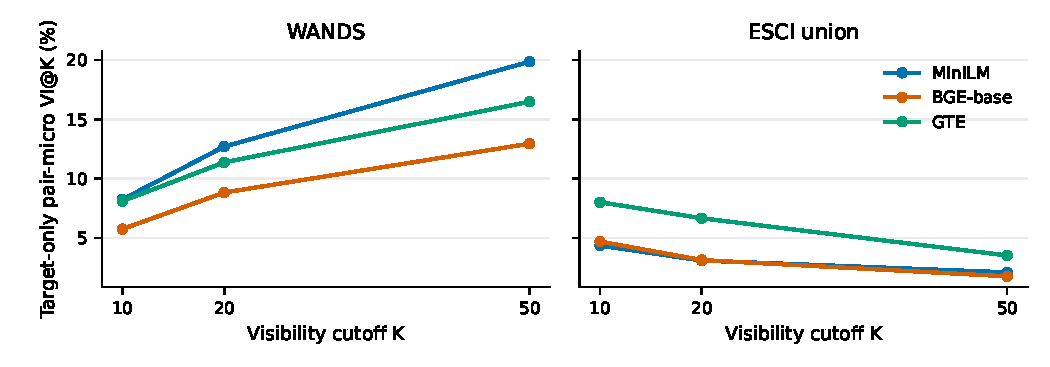
\includegraphics[width=.92\textwidth]{figures/figure5_target_cutoffs.pdf}
\caption{Target-only sensitivity at three visibility boundaries. Each target changes independently; every competitor remains in C0. Points are pair-micro rates, not query-bootstrap estimates. Connecting lines guide the eye and do not interpolate a failure probability.}
\Description{Target-only Top-K crossing fractions at K ten, twenty, and fifty, with separate panels for WANDS and ESCI and curves for MiniLM, BGE, and GTE.}
\label{fig:targetcutoffs}
\end{figure*}

The target-only median rank range is 210, 83, and 105 on WANDS for MiniLM, BGE, and GTE, respectively; on ESCI it is 0, 1, and 2. The zero ESCI median for MiniLM is compatible with nonzero Top-20 instability: most judged relevant pairs can have stable ranks while a smaller subset crosses the boundary. The aggregate result therefore does not depend on asserting that every product moves substantially. Conversely, the much larger WANDS ranges establish movement beyond adjacent swaps without implying that every such movement reaches a user-visible cutoff.

\paragraph{The motivating example across all tested orders.}
Table~\ref{tab:caseorders} exposes every primary serialization for Figure~\ref{fig:example}, including those not selected for the opening illustration. The source-order target is outside Top-20, two tested orders put it inside, and another gets close while remaining outside. The direction is not uniformly favorable. This makes the example a test of nuisance dependence rather than a recommended rewriting policy. The table also shows why fixing competitors matters: the same target score can receive a different rank when the surrounding catalog is reserialized.

\begin{table}[t]
\caption{All orders for the Exact-relevant turquoise chair (MiniLM). Target-only competitors stay in C0. Positive $\Delta$ means a worse rank than target C0.}
\label{tab:caseorders}\centering\small
\begin{tabular}{lrrr}\toprule
Order & Target-only rank & $\Delta$ vs C0 & Catalog-wide rank\\\midrule
C0 & 486 & 0 & 486\\
C1 & 476 & $-10$ & 295\\
C2s1 & 1,527 & $+1,041$ & 1,303\\
C2s2 & 28 & $-458$ & 21\\
C2s3 & 582 & $+96$ & 484\\
C2s4 & 5 & $-481$ & 3\\
C2s5 & 5 & $-481$ & 4\\\bottomrule
\end{tabular}
\end{table}

This case was selected after inspecting the outputs for an intuitive query and a large crossing. It is not an unbiased sample of effect magnitude and cannot substitute for the six aggregate cells. Its scientific role is to make the controlled comparison inspectable: identical facts and fixed competitors can still yield an operationally different result. The population-level inference rests on the full highest-relevance evaluation, not on the visual extremity of this example.

Earlier single-product template interventions provide a complementary check. Replacing only a highest-relevance target with the fact-preserving M1 or M2 representation yields direct top-20 crossing rates of 8.43--10.27\% on WANDS and 7.04--10.80\% on ESCI. Transforming the entire catalog yields rates of 6.13--11.54\%. Rank directions are mixed: representation changes help some relevant items and harm others. The phenomenon is consequently neither a uniform gain nor merely a side effect of every competitor moving at once.

These results motivate relevance--visibility alignment rather than a new average-effectiveness objective. A system may replace one relevant product with another and retain a similar cNDCG, while the first product's opportunity to be retrieved changes sharply. VI identifies that item-level instability; relevance metrics prevent a stable but ineffective representation from counting as a solution.

\subsection{RQ3: Can a Later Ranking Stage Repair the Effect?}

Figure~\ref{fig:pipeline} and Table~\ref{tab:pipeline} separate within-pool movement from first-stage omission. Among products present in every top-100 candidate pool, the cross-encoder approximately halves query-macro VI@20: from 25.94\% to 13.03\% on WANDS and from 3.95\% to 1.37\% on ESCI. Median cross-representation rank range falls from 16 to 8 on WANDS and from 2 to 1 on ESCI. Reranking can therefore correct some ordering among candidates it sees.

\begin{figure}[t]
  \centering
  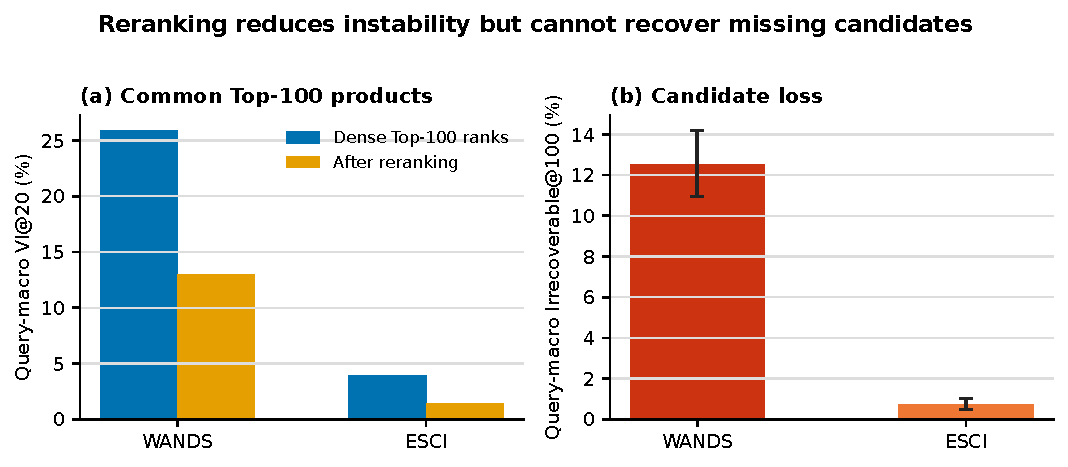
\includegraphics[width=\columnwidth]{figures/figure3_reranker_pipeline.pdf}
  \Description{Bar charts show dense and reranked instability among common candidates, and irrecoverable top-100 loss, for WANDS and ESCI.}
  \caption{Reranking attenuates instability among common candidates (left), but products omitted by first-stage top-100 retrieval are unavailable to the reranker (right).}
  \label{fig:pipeline}
\end{figure}

\begin{table}[t]
\caption{Two-stage BGE--cross-encoder pipeline. VI is query-macro VI@20 on candidates common to all representation pools; loss is query-macro Irrecoverable@100. All values are percentages.}
\label{tab:pipeline}
\centering
\small
\begin{tabular}{lrrr}
\toprule
Data & Dense VI & Rerank VI & Loss (95\% CI) \\
\midrule
WANDS & 25.94 & 13.03 & 12.52 [10.94,14.22] \\
ESCI & 3.95 & 1.37 & 0.72 [0.47,1.00] \\
\bottomrule
\end{tabular}
\end{table}

The remaining failure is structural. Under catalog-wide permutations, 15.14\% of WANDS highest-label pairs enter the top 100 in some variants but are absent in others, producing a 12.52\% query-macro irrecoverable rate. ESCI's rates are lower (0.99\% pair-micro and 0.72\% query-macro) but nonzero. Reranking can correct ordering among candidates, but it cannot recover content it never receives. Candidate generation must therefore remain inside the representation-robustness evaluation boundary.


\paragraph{How many pairs are excluded from the common-pool analysis?}
Table~\ref{tab:coverage} makes the conditioning explicit. On WANDS, 12,240 highest-relevance pairs appear in at least one top-100 pool, but only 8,384 occur in every pool. The difference, 3,856 pairs, is the representation-dependent candidate-loss population. On ESCI, the corresponding counts are 4,039 and 3,995, a difference of 44. These are query--product pairs rather than unique products: the same catalog item can be relevant to multiple queries.

\begin{table}[t]
\caption{Candidate coverage under catalog-wide BGE permutations. ``Some only'' is ever retrieved minus common to all pools. The conditional loss divides that count by ever retrieved; it is distinct from the all-highest and query-macro rates.}
\label{tab:coverage}\centering\small
\begin{tabular}{lrr}\toprule
Population & WANDS & ESCI\\\midrule
All highest-relevance pairs & 25,470 & 4,434\\
Ever in Top-100 & 12,240 & 4,039\\
In every Top-100 & 8,384 & 3,995\\
Some pools only & 3,856 & 44\\
Loss conditional on ever retrieved & 31.50\% & 1.09\%\\\bottomrule
\end{tabular}
\end{table}

The conditional rate is useful because it asks about relevant content that the retriever demonstrates it can retrieve under at least one equivalent input. For WANDS this is 31.50\%; for ESCI it is 1.09\%. These values must not replace the primary all-highest rates without changing the claim. Pairs absent under every serialization are outside this conditional denominator and contribute zero to representation-induced crossing even though their persistent omission can still be a retrieval-effectiveness problem.

There is also a selection effect in evaluating only common candidates. Membership in every pool removes the very products whose availability is unstable at the first-stage boundary. The reduced VI after reranking is therefore evidence about ordering conditional on survival, not a complete end-to-end robustness guarantee. Reporting both candidate coverage and conditional reranker stability prevents this survivorship restriction from being mistaken for recovery of missing content.

For additional context, C0 highest-label Recall@20 rises from 12.58\% to 13.61\% after reranking on WANDS and from 68.04\% to 70.37\% on ESCI. These stored C0 point estimates show that improved relevance retrieval and residual representation instability can coexist. They are not paired significance claims, and their cross-dataset difference reflects distinct catalogs and relevance populations. The key pipeline conclusion concerns availability: a later ranker can improve a candidate's position only when that candidate has reached it.

\subsection{RQ4: Can Robustness Improve Without Sacrificing Relevance?}

Table~\ref{tab:mitigation} compares the set-mean proof of concept with two deterministic baselines. Canonical sorting (M2) mechanically collapses permutations and obtains VI=0, but causes a confirmed held-out WANDS cNDCG@10 decrease of 0.0217. The factual template (M1) leaves residual instability and has a smaller confirmed WANDS decrease of 0.0069. Set mean also obtains VI=0 and changes WANDS cNDCG by $-0.0096$, with a paired 95\% CI from $-0.0195$ to $0.0003$. On ESCI, its change is $-0.0066$, with a CI from $-0.0187$ to $0.0055$.

\begin{table}[t]
\caption{Robustness--relevance comparison with BGE. Values are cNDCG@10; parentheses show paired change from Original. WANDS contains the held-out 80\%. Macro VI is a percentage.}
\label{tab:mitigation}
\centering
\small
\begin{tabular}{llrr}
\toprule
Data & Method & cNDCG@10 ($\Delta$) & Macro VI \\
\midrule
\multirow{4}{*}{WANDS}
 & Original & .8247 & 11.93 \\
 & M1 factual & .8178 ($-.0069$) & 11.23 \\
 & M2 canonical & .8030 ($-.0217$) & 0 \\
 & Set mean & .8151 ($-.0096$) & 0 \\
\midrule
\multirow{4}{*}{ESCI}
 & Original & .7124 & 3.66 \\
 & M1 factual & .7061 ($-.0063$) & 3.08 \\
 & M2 canonical & .7192 ($+.0068$) & 0 \\
 & Set mean & .7059 ($-.0066$) & 0 \\
\bottomrule
\end{tabular}
\end{table}

Set mean's maximum score difference across permutations is $2.38\times10^{-7}$, below the prespecified $10^{-6}$ numerical tolerance. The set-based representation thus eliminates measured order-induced instability, while the observed retrieval-effectiveness change is small and statistically inconclusive on both evaluation sets. This does not prove equivalence: the WANDS interval still permits a meaningful loss. The result instead identifies a promising point on a robustness--relevance frontier (Figure~\ref{fig:pareto}) and shows why stability and relevance must be evaluated jointly.

\begin{figure}[t]
  \centering
  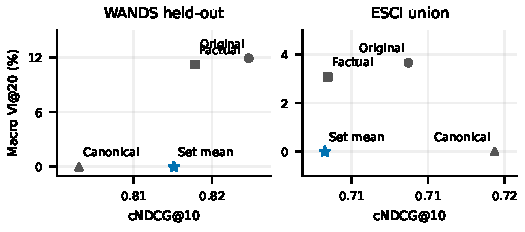
\includegraphics[width=\columnwidth]{figures/figure4_pareto.pdf}
  \Description{Scatter plots place original, factual, canonical, and set-mean representations by cNDCG and visibility instability on WANDS and ESCI.}
  \caption{Robustness--relevance frontier. Lower VI and higher cNDCG are preferred. Effectiveness intervals for all variants appear in Figure~\ref{fig:effectivenessci}.}
  \label{fig:pareto}
\end{figure}


\paragraph{Inspecting the effectiveness uncertainty.}
Figure~\ref{fig:effectivenessci} adds paired confidence intervals for all evaluated mitigation variants. It complements the robustness--relevance scatter plot by exposing the uncertainty that a point-only frontier cannot show. Set mean's interval crosses zero on both datasets, but much of the WANDS interval lies on the loss side. Calling this ``no loss'' would conflate failure to establish a difference with evidence that the difference is negligible. A deployment decision would require a prespecified acceptable-loss margin and a study designed to assess that margin.

\begin{figure*}[t]
\centering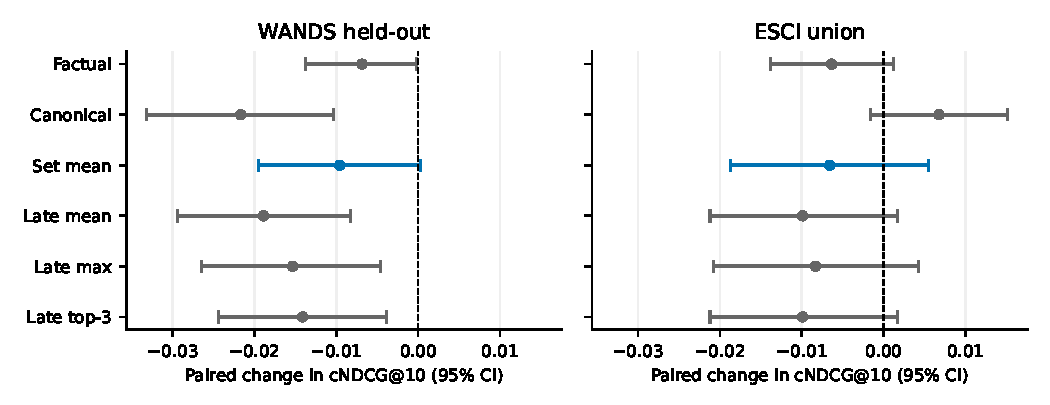
\includegraphics[width=.92\textwidth]{figures/figure6_effectiveness_intervals.pdf}
\caption{Paired effectiveness changes relative to Original, with stored 95\% confidence intervals. The dashed line denotes zero change, not an equivalence margin. Set mean is highlighted; the late-aggregation negative results remain visible.}
\Description{Confidence intervals for six representation methods on held-out WANDS and ESCI. Set-mean intervals span zero on both; the late variants have entirely negative WANDS intervals.}
\label{fig:effectivenessci}
\end{figure*}

\paragraph{What the negative variants teach us.}
All late-aggregation variants satisfy the numerical order-invariance criterion, yet on held-out WANDS their cNDCG@10 values are 0.8058, 0.8093, and 0.8106 for late mean, maximum, and top-3 aggregation. Each paired interval establishes a decrease relative to Original. On ESCI their values are 0.7026, 0.7041, and 0.7026, with intervals spanning zero. Thus invariance does not determine effectiveness: the aggregation rule still controls which aspects of a structured record dominate matching.

Canonical sorting makes the same point from another direction. It obtains zero measured instability but loses effectiveness on WANDS, whereas its ESCI point estimate is higher than Original without a confirmed gain. The available evidence does not establish a universal ranking of the invariant approaches. In particular, a significant Original-versus-canonical contrast and an inconclusive Original-versus-set-mean contrast do not establish that set mean significantly outperforms canonical sorting. Such a claim would require their direct paired comparison.

The useful outcome is therefore a design constraint and a proof of feasibility within the tested family. A representation can remove dependence on attribute order while retaining substantial relevance effectiveness, but the relevance cost must be measured rather than assumed away. Further optimization should preserve this two-objective evaluation, including unsuccessful variants, so that apparent robustness gains cannot be obtained simply by erasing information needed for matching.
